\subsection{Rectangle-line picking}
\label{sec:rectangle_line}

Here we consider choosing lines from a rectangle with side lengths $a$
and $b$, which we order $a \leq b$ (without loss of generality).  We
also describe the problem by the aspect ratio of the rectangle, i.e.,
$a \!: \!b$, assuming the length of the diagonal $L=\sqrt{a^2+b^2}$ is
given. 

Chosing random end-points from the rectangle is no harder than for the
square -- we simply choose (independently) $x_i \sim U(0,b)$, and $y_i
\sim U(0,a)$. Figure~\ref{fig:rect_eg} shows an example.

Figure~\ref{fig:rect_pdf} shows the PDF for the rectangle,
highlighting the different regions with shaded colours and
Table~\ref{tab:summary_line} shows the basic statistics, though in
some places the formulae are too complicated to fit in the table, and
we only provide references.

\begin{figure}[htbp]
  \begin{center}
    \subfloat[\label{fig:rect_eg}Example.]{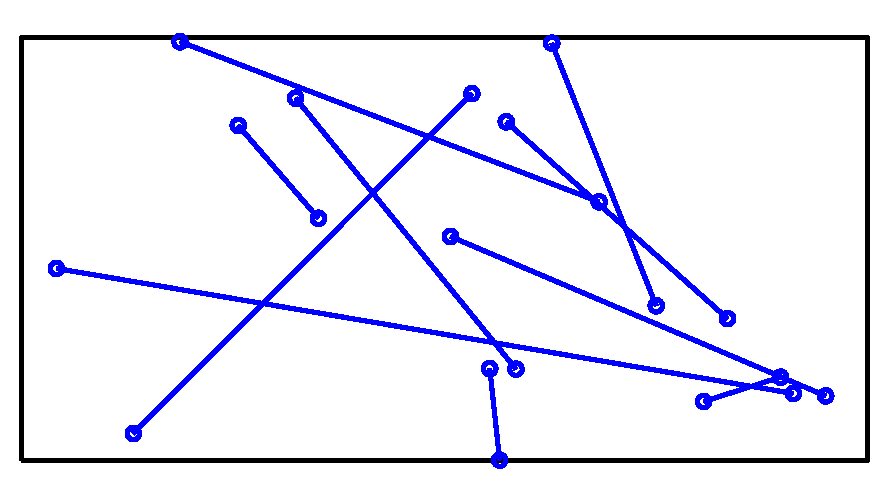
\includegraphics[width=0.3\columnwidth]
          {../Matlab/Plots/LinePicking_eg_rect.eps}} 
       \hspace{0.075\columnwidth}
    \subfloat[\label{fig:rect_pdf}PDF (aspect ratio 1:1.2) showing regions.]{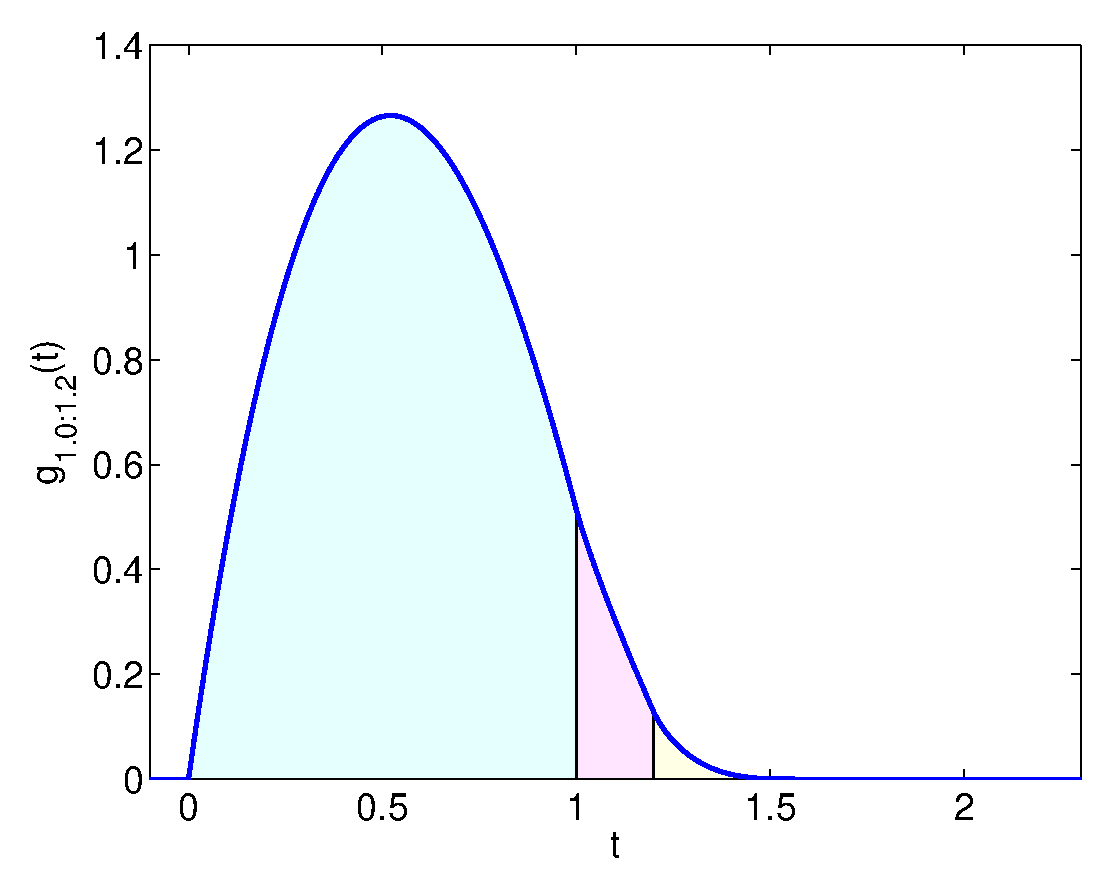
\includegraphics[width=0.5\columnwidth]
          {../Matlab/Plots/LinePicking_plot_rect_regions.eps}}
    \caption{The rectangle line-picking problem ($L=\sqrt{a^2+b^2}=\sqrt{2}$).}
  \end{center} 
\vspace{-4mm}
\end{figure}

\begin{table}[ht]
  \centering
  \begin{tabular}{|r|c|l|}
    \hline
    Statistic & Value & Source \\ 
    \hline
      Support            & $t \in [0, L]$ & \\
      PDF                & See \eqref{eqn:rectangle} and \eqref{eqn:rectangle2}   &
                             \cite{b.ghosh51:_random_rect,mathai_geom} \\
      CDF                & See \eqref{eqn:rectangle_cdf}. & 
                           \eqref{eqn:rectangle_cdf} \\
      $i$th Moment $m_i$ & First 4 are given in
      \eqref{eq:rect_moments}-\eqref{eq:rect_moments_end}. 
                        & \cite{b.ghosh51:_random_rect} \\
      Mean               & See \eqref{eq:rect_moments}. &
                             \cite{} \\[1.5ex]
      Variance           & $\displaystyle m_2 - m_1^2$ &
                             \cite{} \\[1.5ex]
    \hline
  \end{tabular}
  \caption{Summary of the rectangle-line picking problem for $L=\sqrt{a^2+b^2}$.}
  \label{tab:summary_line}
\end{table}

\subsubsection{PDF}

The PDF for the rectangle is given in 
\cite[Theorem 2.4.4]{mathai_geom} and 
\cite[Theorem 2]{b.ghosh51:_random_rect}
\begin{equation}
  g^{\rm rect}_{a,b}(t) = \frac{4 t}{a^2 b^2} \phi_{a,b}(t),
  \label{eqn:rectangle}   
\end{equation}
where
\begin{equation}
  \phi_{a,b}(t) = \left\{
    \begin{array}{ll}
      \frac{ab \pi}{2} - (a+b) t + \frac{t^2}{2}, 
         & \mbox{ for } t \leq a, \\
      a b \sin^{-1} (a/t) - \frac{a^2}{2} - b t + b\sqrt{t^2 - a^2},
         & \mbox{ for } a \leq t \leq b, \\
      a b \left[ \sin^{-1} (a/t) - \sin^{-1} \sqrt{1 - \frac{b^2}{t^2}} \right]
        - \frac{a^2 + b^2 + t^2}{2} 
        + a\sqrt{t^2 - b^2}+ b\sqrt{t^2 - a^2},
         & \mbox{ for } b \leq t \leq \sqrt{a^2 + b^2}, \\
      0,
         & \mbox{ otherwise}, \\
    \end{array} \right. 
  \label{eqn:rectangle2}   
\end{equation}
where the rectangle has sides of length $a \leq b$.

This is a rather complicated expression, but is easily evaluated
numerically.  Naldi \cite{m.naldi05:_connec_of_waxman_graph}
approximated this expression with a $\beta$ function, though given the
requirements to numerically evaluate that function there hardly seems
any advantage, though we shall see later that this would have been
completely appropriate if the region have been a disk.

Figure~\ref{fig:rect_pdf_var} shows a comparison of the PDFs for
rectangles with varying aspect ratios, chosen such that $L = \sqrt{a^2
  + b^2} = 1$ to allow easy comparison. We can see that for longer,
thinner rectangles, the PDF is comprised of two main segments: (i) a
part approximating the shape of that for the square (though compressed
into a short range of values of $t$), and (ii) an almost straight
component, similar to the PDF for line-line picking problem. The
reasons for this also seem relatively intuitive.

\begin{figure}[htbp]
  \begin{center}
    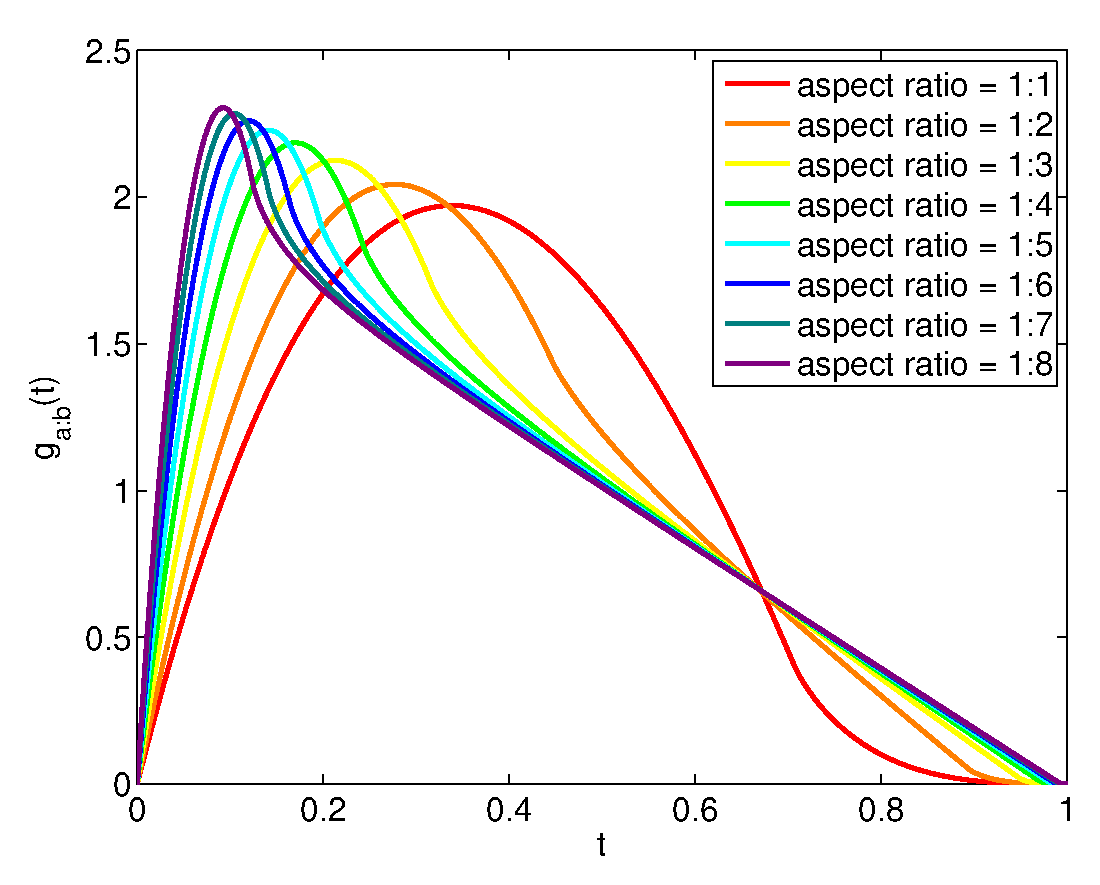
\includegraphics[width=0.5\columnwidth]
          {../Matlab/Plots/LinePicking_plot_rect.eps}
    \caption{PDF of rectangles with various aspect
              ratios (and fixed $L=1$).}
    \label{fig:rect_pdf_var}
  \end{center} 
\vspace{-4mm}
\end{figure}

We can calculate the limit as $a \rightarrow 0$ to see the PDF for the
line-line picking problem.  We keep $a^2 + b^2 = L^2$ so that the
support of the PDF remains constant.  As $a \rightarrow 0$, we only
need consider the case $a \leq t \leq b$, where
\begin{eqnarray}
    g^{\rm rect}_{a,b}(t)
        & = & \frac{4 t}{a^2 b^2} 
                  \left[ a b \sin^{-1} (a/t) - \frac{a^2}{2} - b t + b\sqrt{t^2 - a^2} \right] , \nonumber \\
        & \simeq & \frac{4t }{a b} \sin^{-1} (a/t)
                   - \frac{2 t}{b^2}
                    + \frac{4 t}{a^2 b^2} \left[ -b t + b t - \frac{b a^2}{2 t} \right] , \nonumber \\
        & \simeq & \frac{2}{b}
                   - \frac{2 t}{b^2}, 
\end{eqnarray}
where we have used the following Taylor series around $x=0$, dropping
the higher order terms:
\[ \sin^{-1}(x) = x + \frac{x^3}{6} + \cdots, 
   \mbox{ and }
   \sqrt{t^2 - x^2} = t - \frac{x^2}{2t} - \frac{x^4}{8 t^3} \cdots .
\]
The result just returns to the line-line picking PDF.

\subsubsection{CDF}

The PDF has long been given, but as far as we can tell, the CDF has
never been written explicitly.  The CDF can be derived by integration
of the PDF, but we derived it here more directly by ...

\begin{equation}
  G^{\rm rect}_{a,b}(t)  = \left\{
    \begin{array}{ll}
     \frac{t^2}{6 a^2 b^2} \left( 
       6 a b \pi - 8(a+b) t + 3 t^2
             \right),  
         & \mbox{ for } t \leq a, \\
     \frac{1}{6 a^2 b^2} \Big( 
       (ab + 8 b \left( \sqrt{t^2 - a^2} -t \right) t^2
          - a^2 \left( 6 t^2 - 4 b  \sqrt{t^2 - a^2} \right)
          + 12 a b t^2 \sin^{-1}(a/t)
             \Big),  
         & \mbox{ for } a \leq t \leq b, \\
     \frac{1}{6 a^2 b^2} \Big( 
         a^4 + b^4
        + 4 a \sqrt{t^2 - b^2} (b^2 + 2 t^2)
        + a^2 (-6 t^2 + 4 b \sqrt{t^2 - a^2}) & \\
        + \hspace{5mm} t^2 (-6 b^2 - 3 t^2 + 8 b \sqrt{t^2 - a^2})
        + 12 a b t^2 \left( 
                       \sin^{-1}(b/t) - \pi/2 + \sin^{-1}(a/t)
                     \right)
      \Big),
         & \mbox{ for } b \leq t \leq \sqrt{a^2 + b^2}, \\
    \end{array} \right. 
  \label{eqn:rectangle_cdf}   
\end{equation}


\subsubsection{Moments}

Ghosh \cite{b.ghosh51:_random_rect} gives the first four moments of
the line-length distribution for the rectangle
\begin{eqnarray}
  \label{eq:rect_moments} 
  m^{\rm rect}_1 & = & \frac{1}{6} \left[ 
                        \frac{b^2}{a} \cosh^{-1}\left( L/b \right) +
                        \frac{a^2}{b} \cosh^{-1}\left( L/a \right) 
                 \right]
                  + \frac{1}{15} \left[ \frac{a^3}{b^2} + \frac{b^3}{a^2} \right]
                  - \frac{L}{15} \left[ \frac{a^2}{b^2} + \frac{b^2}{a^2} -3 \right],
\\
  m^{\rm rect}_2 & = & \frac{1}{6} L^2, \\
  m^{\rm rect}_3 & = & \frac{1}{20} \left[ 
                        \frac{b^4}{a} \cosh^{-1}\left( L/b \right) +
                        \frac{a^4}{b} \cosh^{-1}\left( L/a \right) 
                 \right]
                  + \frac{2}{105} \left[ \frac{a^5}{b^2} + \frac{b^5}{a^2} \right]
                  - \frac{2L}{105} \left[ \frac{a^4}{b^2} + \frac{b^4}{a^2}\right]
                        - \frac{5}{84} L^3, 
\\
  m^{\rm rect}_4 & = & \frac{1}{15} a^4 + \frac{1}{18} a^2 b^2 + \frac{1}{15} b^4,
  \label{eq:rect_moments_end} 
\end{eqnarray}
where $L = \sqrt{a^2 + b^2}$, from which we can derive the special
cases of the square and line (though these can also be derived
directly). Obviously central moments such as mean, and variance, etc.,
can be derived immediately from these, though the formulae are
complicated and unelightening.
